\chapter{Results\label{chap:results}}

This section covers a comparison of the image processing techniques, a CIV performance analysis for the differently processed images and the analysis of the resulting wind fields.

\section{Comparison of Image Processing Techniques}
\FloatBarrier
\begin{figure}[h!] 
    \centering
    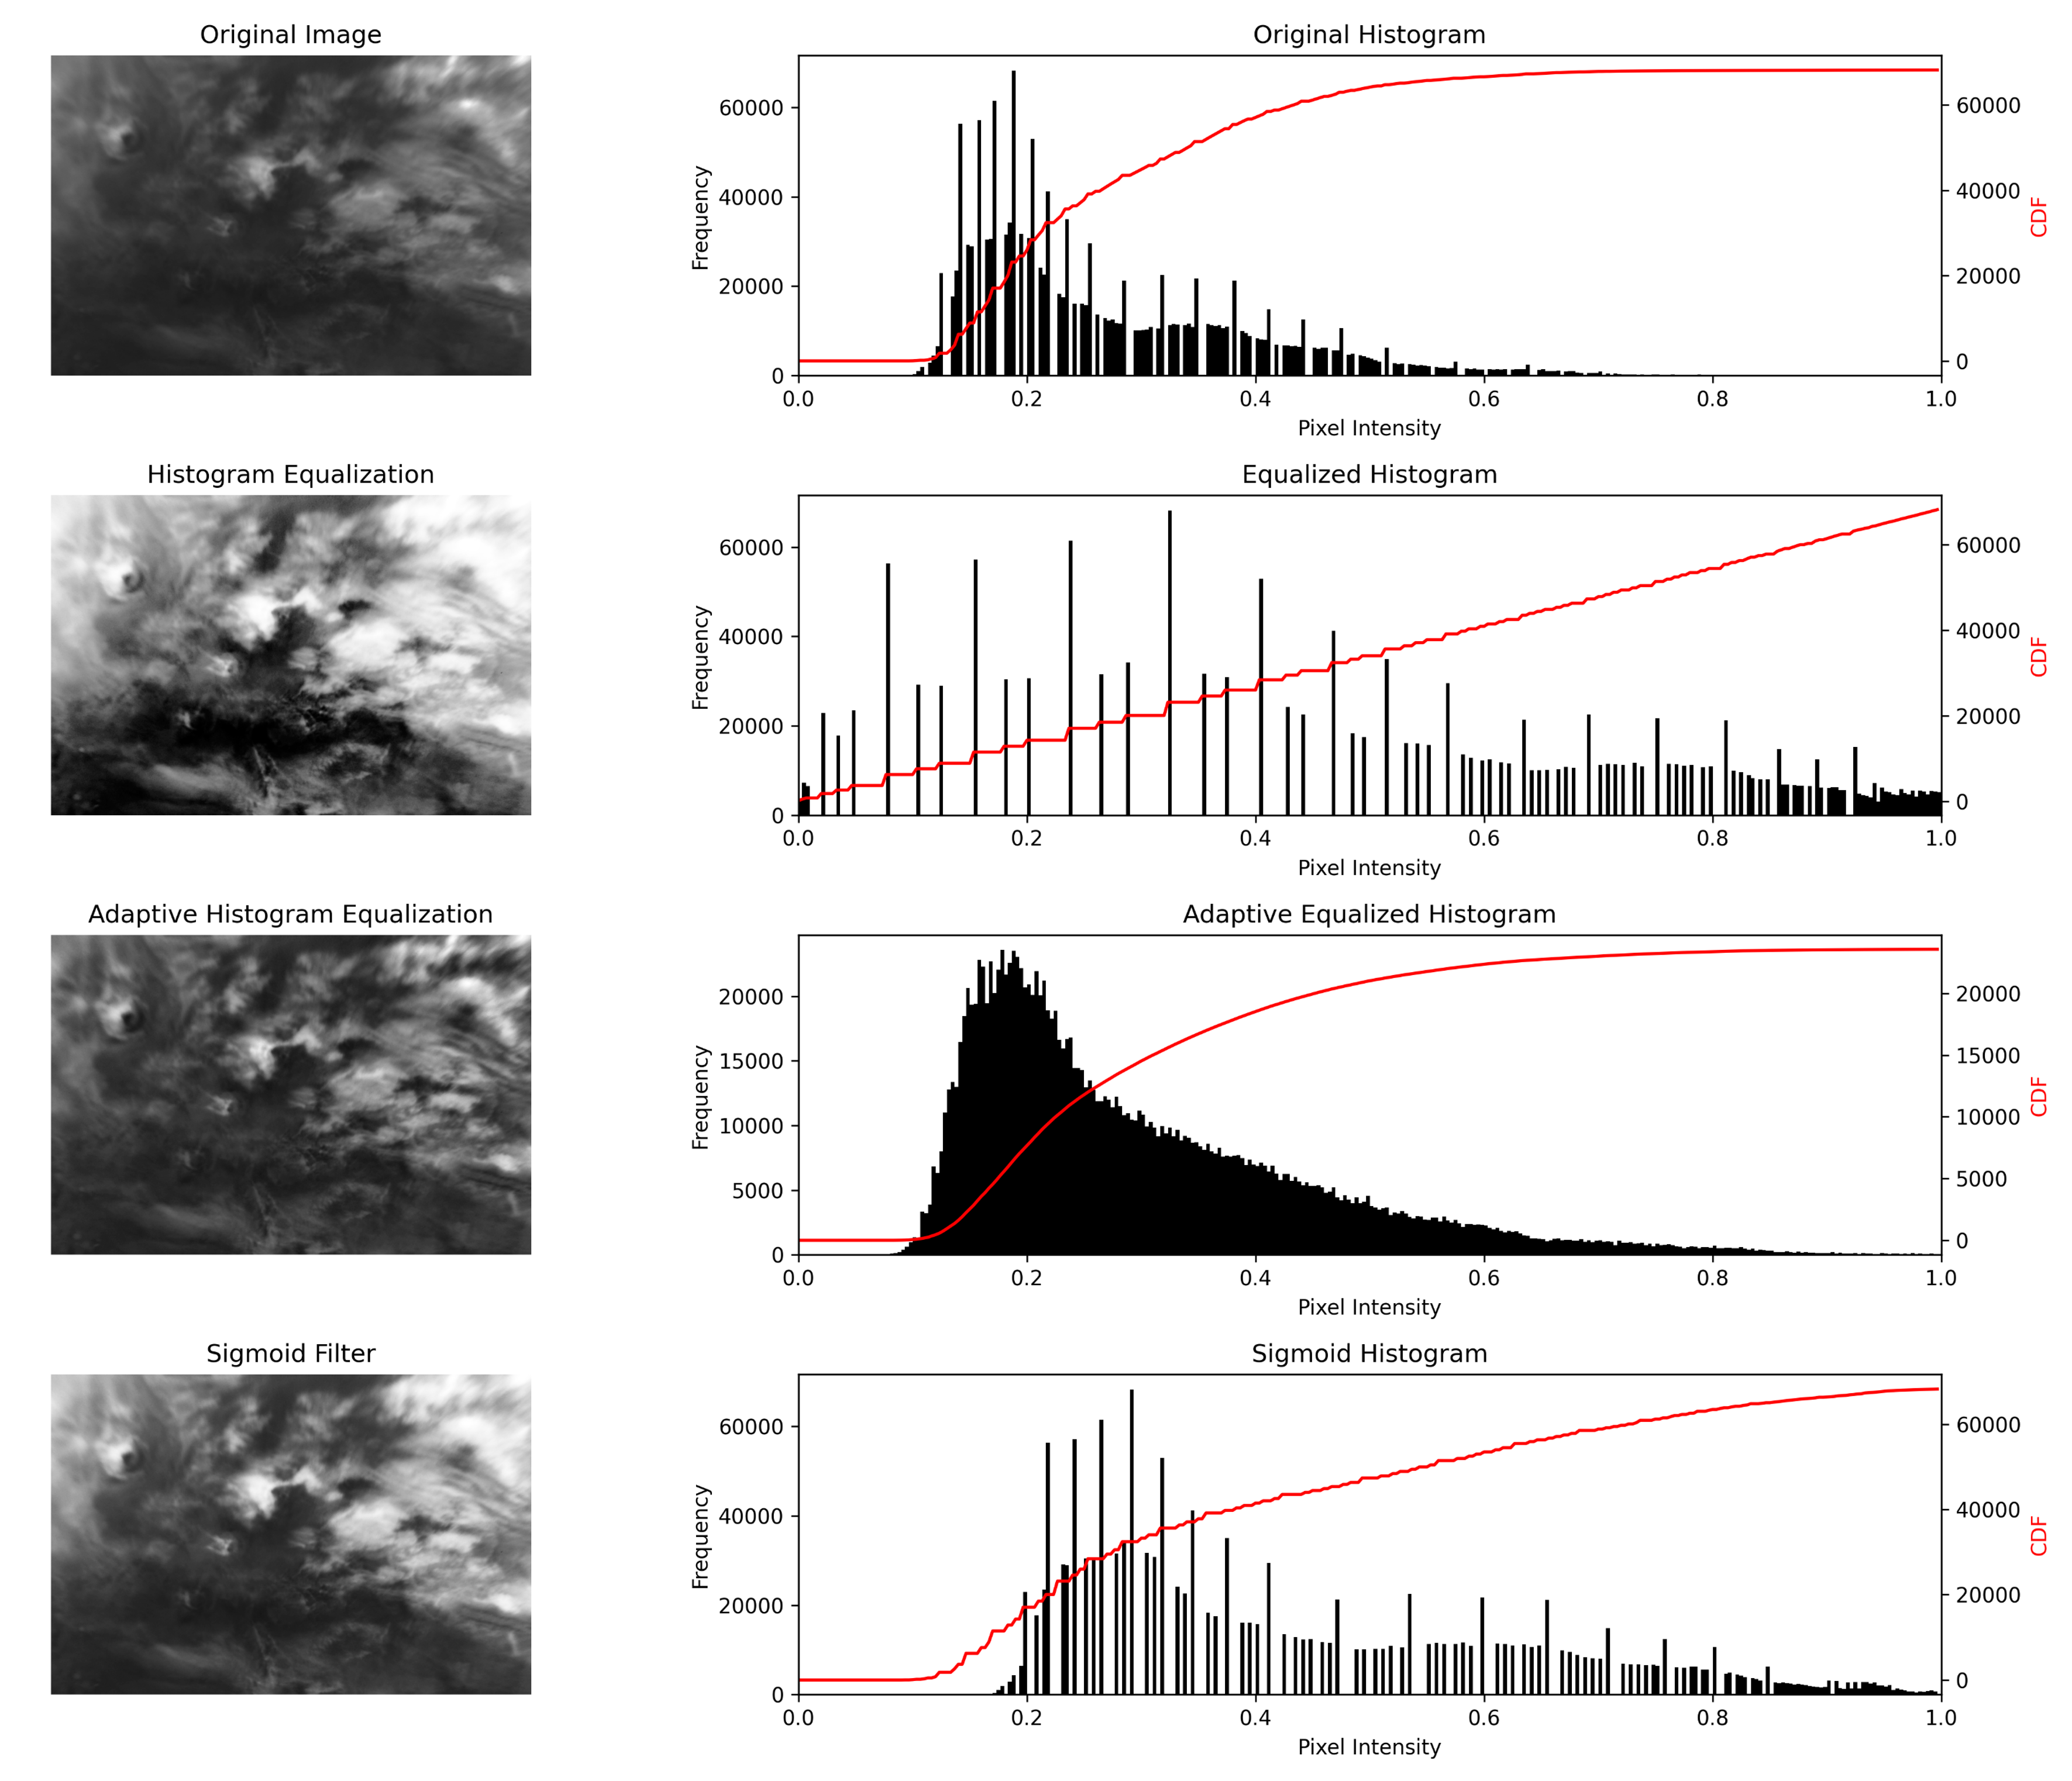
\includegraphics[width=0.9\textwidth]{fig_31.png}
    \caption{overview of differently processed image versions from UTC: 22/11/2021 14:16:52.}
\end{figure}
\FloatBarrier
When comparing the visual results of the image enhancement methods (see Figure 4.1), the sigmoid filter stands out as particularly effective. It enhances the images by brightening them to reveal clouds that were visually hidden in darker pixels, without over-intensifying the lighter areas. In contrast, HE tends to overemphasize bright pixels, leading to high contrast that obscures fine details. CLAHE performs somewhat better, however, potentially results in a disproportionate representation of intensity levels in sub-regions.

As evidenced by the histogram and CDF, the sigmoid filter appears to preserve the original data more effectively. The histogram shows maintains its original shape but shifts to the right. Similarly, the CDF remains similar although flattened.

\section{CIV - Performance Comparison}

After performing CIV on the differently processed images, the average correlation coefficient  after removal of warning and error flags and the percentage of warning and error flags were analysed.
\FloatBarrier
\begin{figure}[h!] 
    \centering
    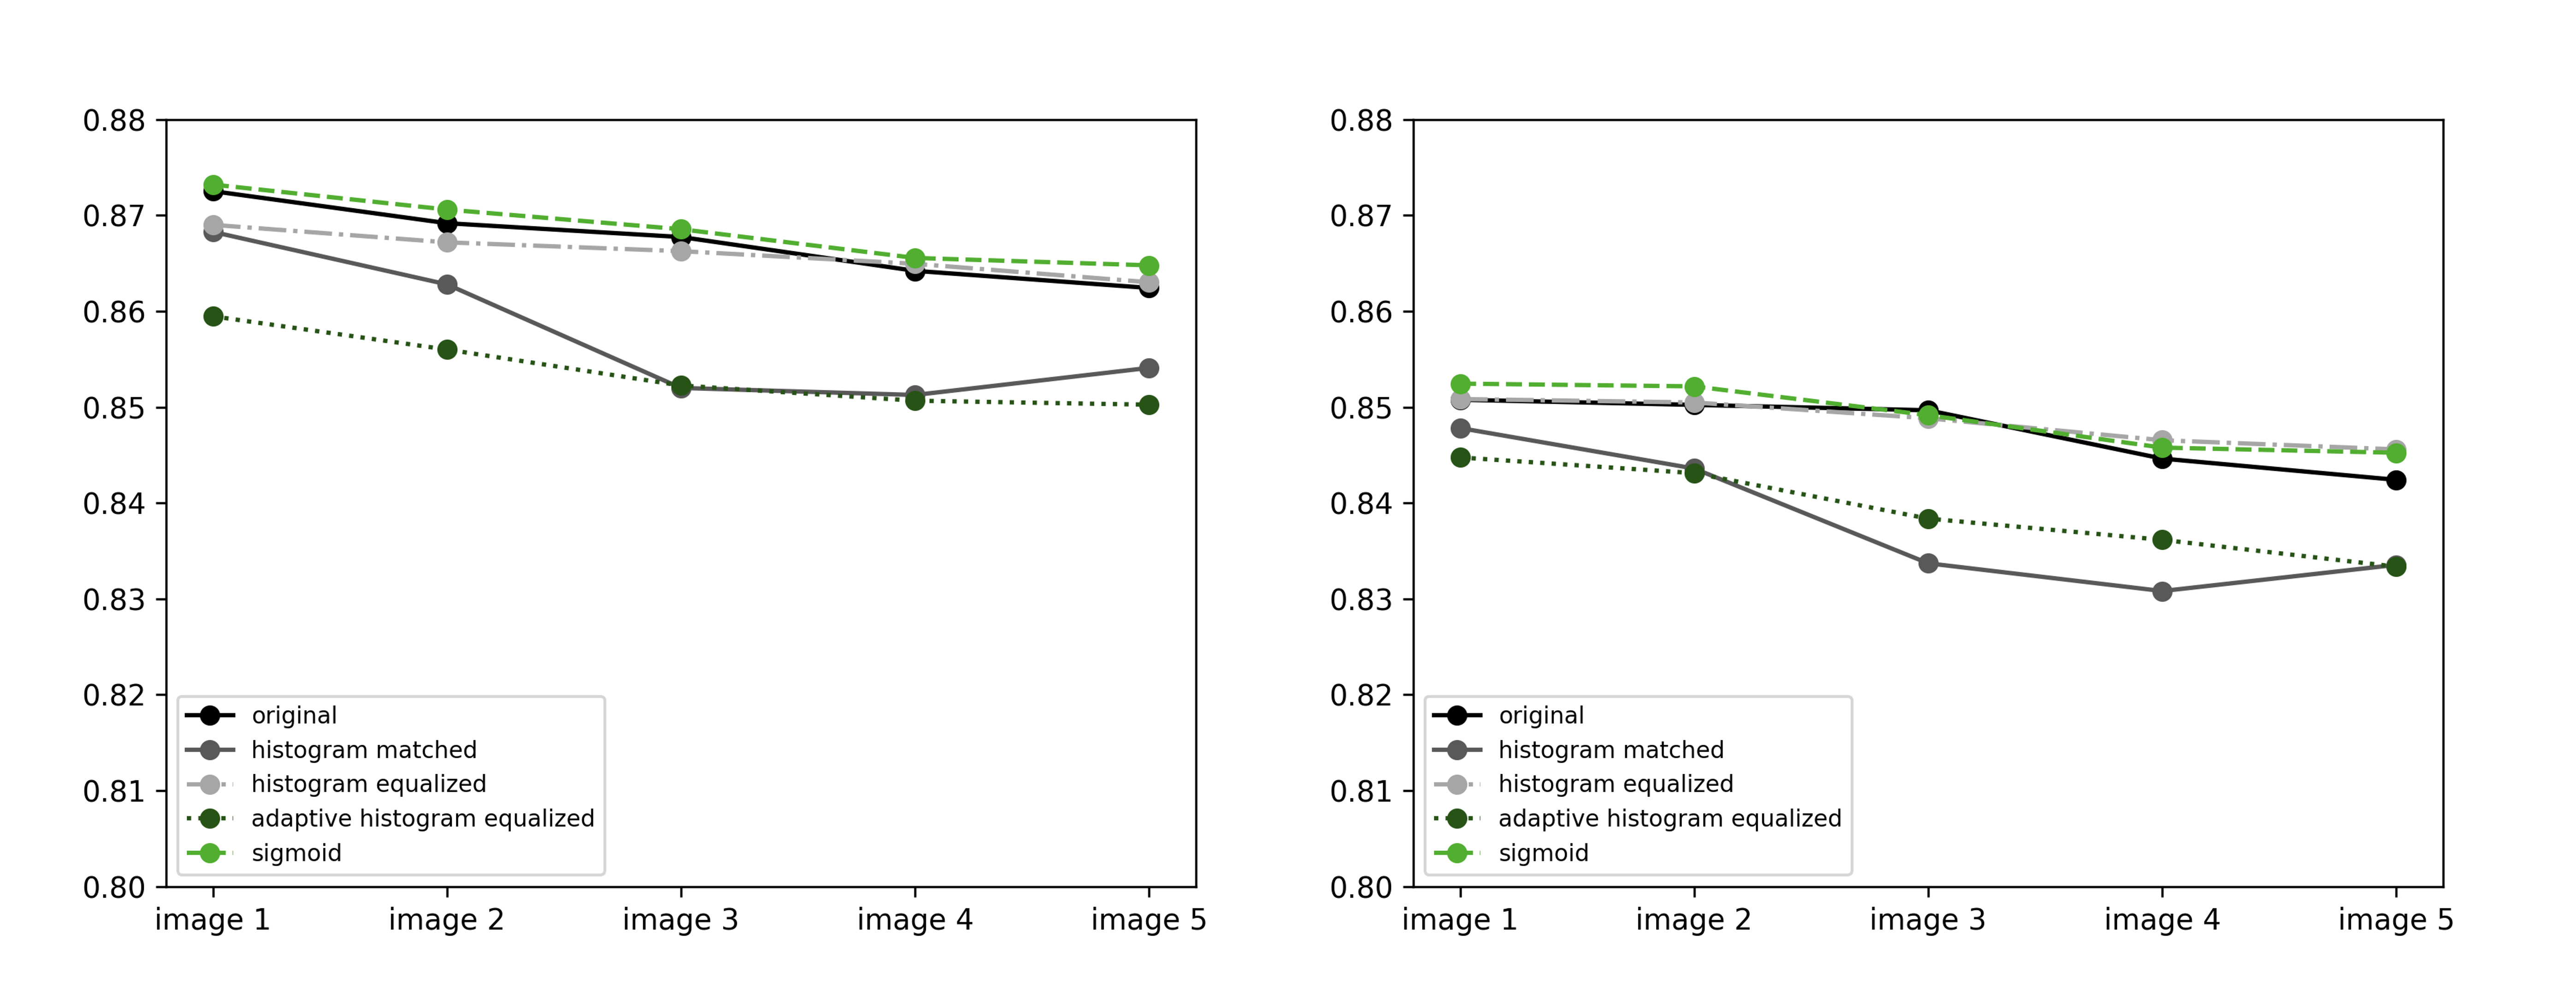
\includegraphics[width=1\textwidth]{fig_32.png}
    \caption{Plot of the average correlation co-efficient of vector fields identified during CIV1 (left) and CIV2 (right) for each image transition. Vectors with error flags were removed before the calculation. The data source of this visualisation are 6 images from 24/12/2021 ranging over the time span 10:30:07 - 11:20:06 with a time separation of 10 minutes.}
\end{figure}
\FloatBarrier
The average correlation co-efficient determined during the CIV process across each image sequence is generally high at around 0.8, however, different image processing techniques lead to changes in the performance (as displayed in figure 4.2). 
Analysing the CIV results of each image sequence, the original, sigmoid transformed and HE images have a higher average correlation co-efficient than the histogram matched and CLAHE images.
\FloatBarrier
\begin{figure}[h!] 
    \centering
    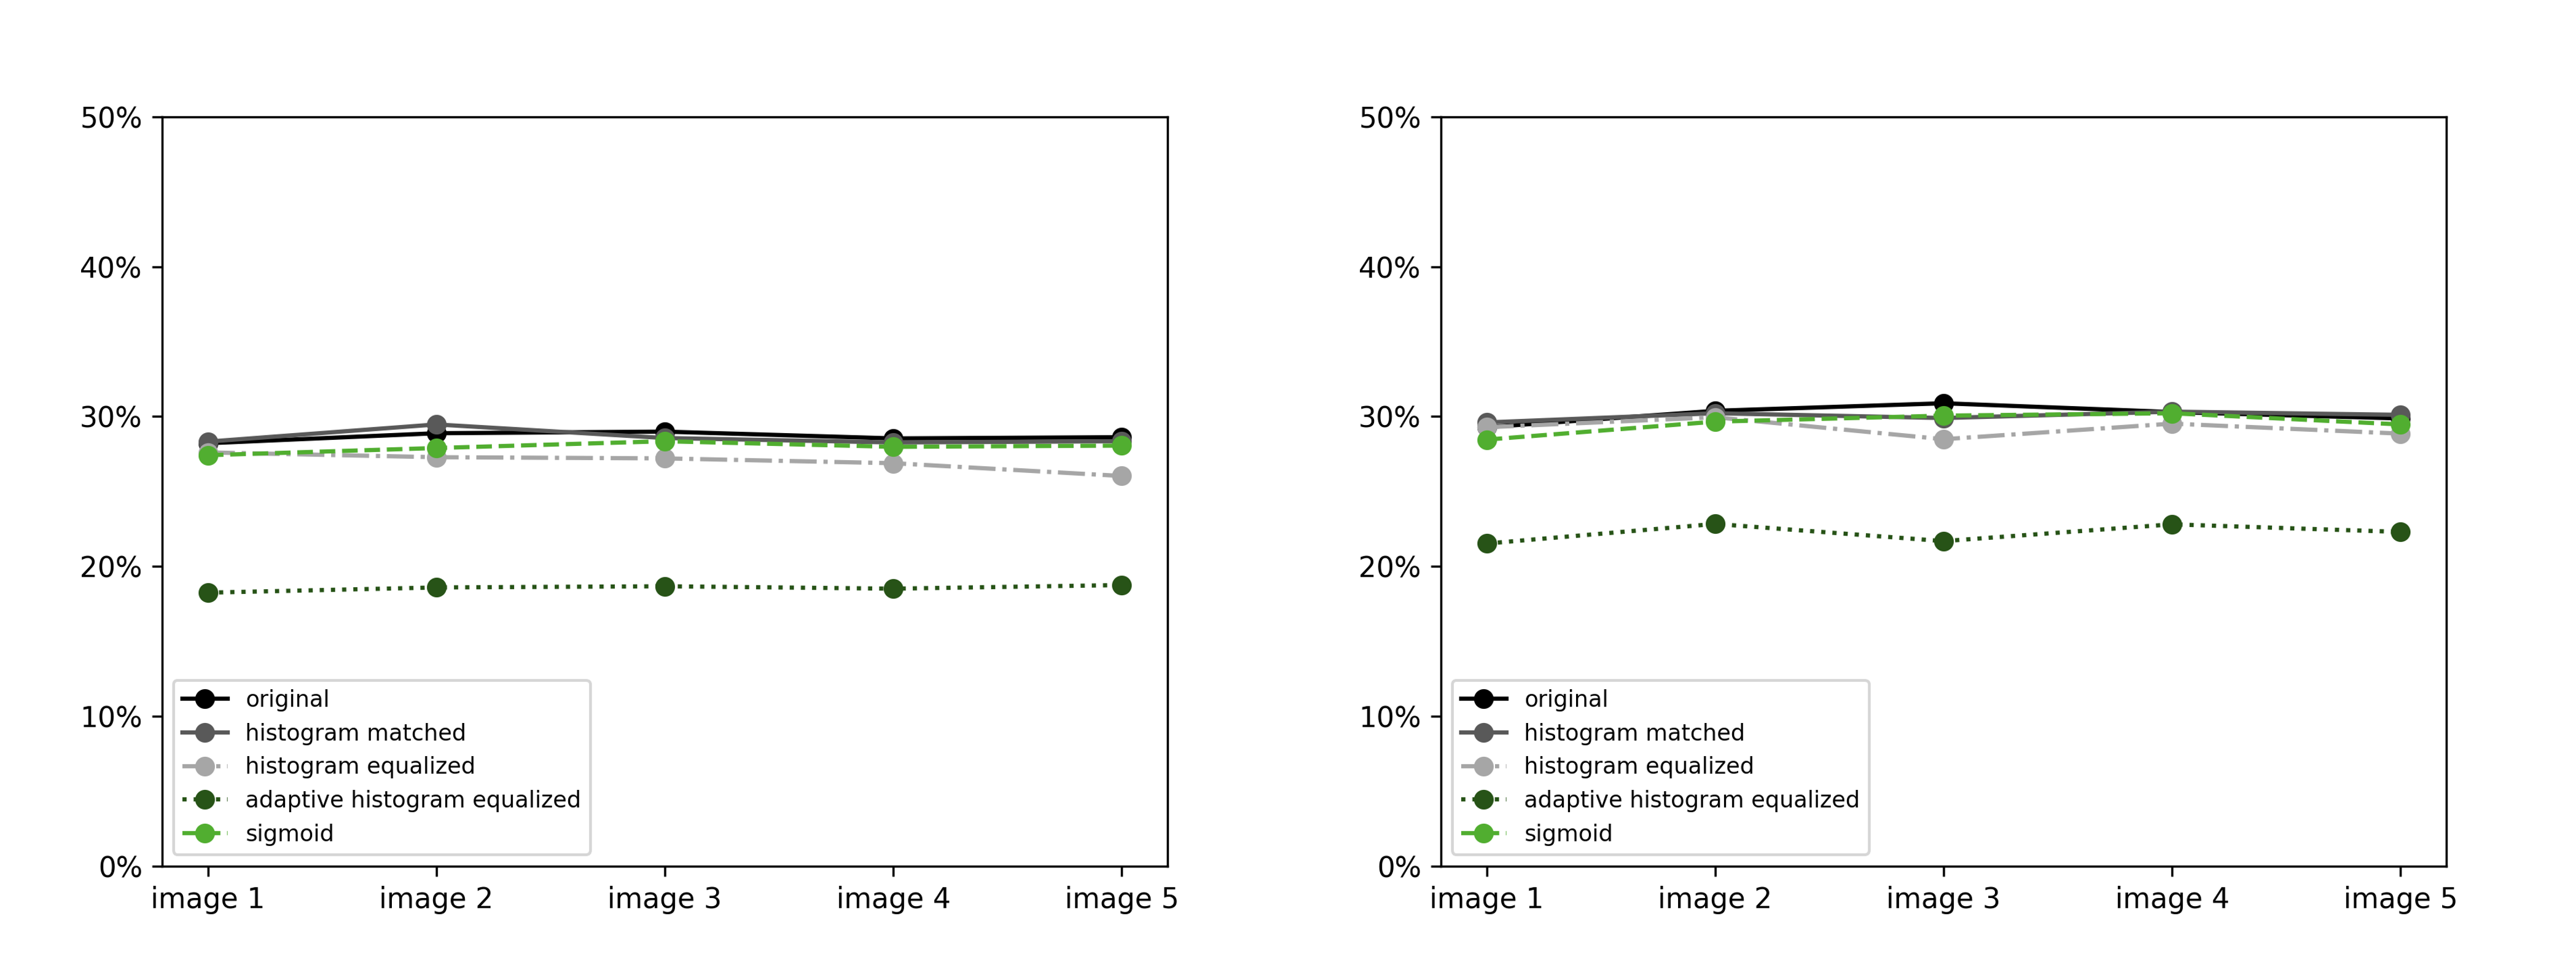
\includegraphics[width=1\textwidth]{fig_33.png}
    \caption{Plot of the amount FF errors displayed in percentages of the total number of vectors identified during CIV1 (left) and CIV2 (right) for each image transition. The data source of this visualisation are 6 images from 24/12/2021 ranging over the time span 10:30:07 - 11:20:06 with a time separation of 10 minutes.}
\end{figure}
\FloatBarrier
The percentages of FF error flags (see Figure 4.3), which highlight irregularities in the calculation of velocity vectors\cite{TutorialUVMAT}, are relatively consistent across most methods, except for CLAHE. 
The reduced occurrence of false vectors in CLAHE-processed images might be attributed to the suppression of noise and improved visibility of features. The reduced number of error flags in CLAHE-processed sequences may contribute to the lower correlation coefficient, due to the presence of additional velocity vectors, lowering the overall average.
\FloatBarrier
\begin{figure}[h!] 
    \centering
    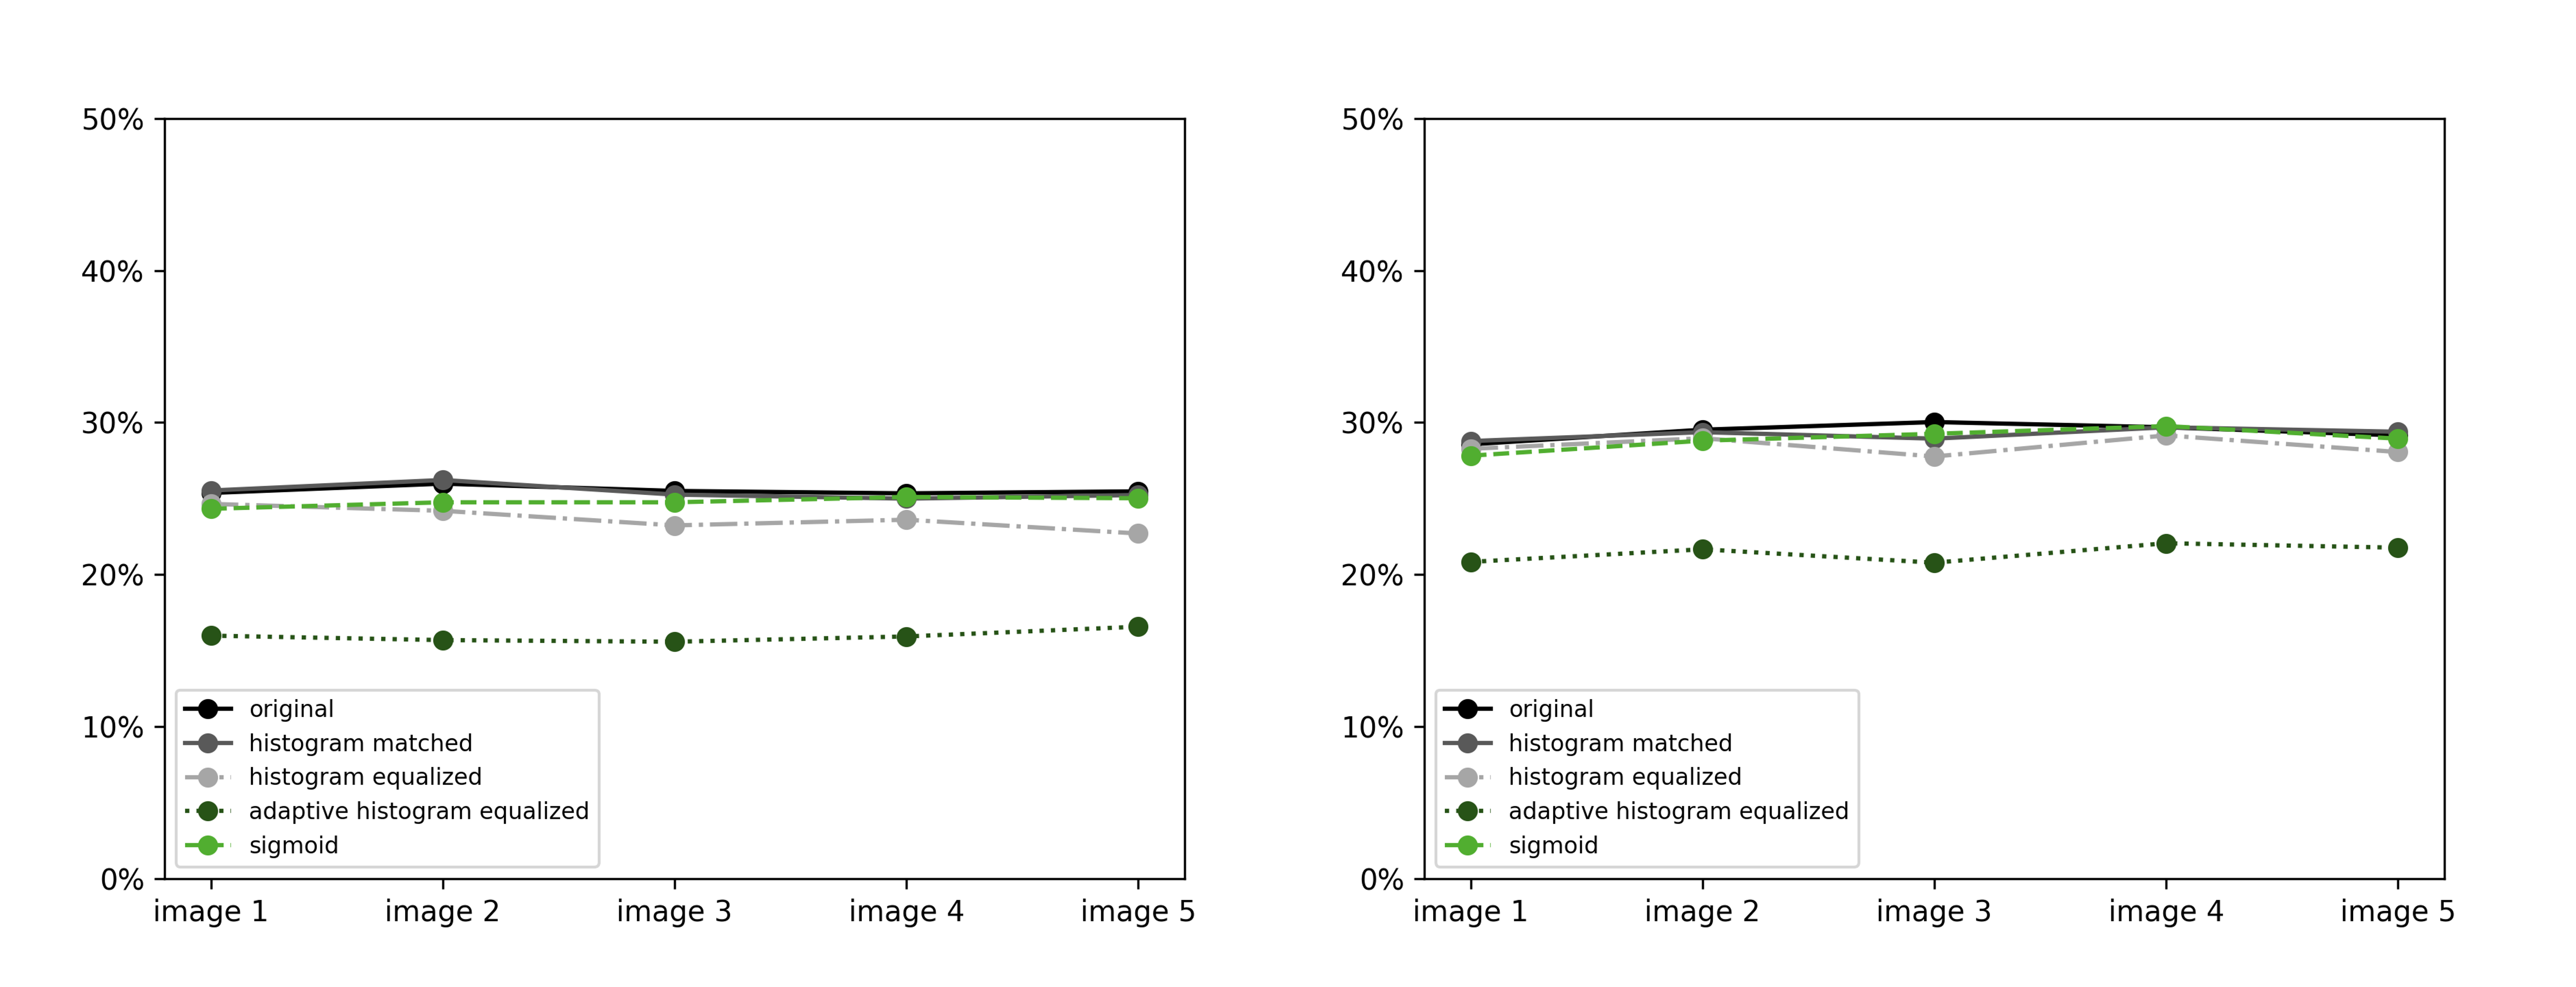
\includegraphics[width=1\textwidth]{fig_34.png}
    \caption{Plot of the amount F warnings displayed in percentages of the total number of vectors identified during CIV1 (left) and CIV2 (right) for each image transition. The data source of this visualisation are 6 images from 24/12/2021 ranging over the time span 10:30:07 - 11:20:06 with a time separation of 10 minutes.}
\end{figure}
\FloatBarrier
F warning flags (as shown in Figure 4.4) usually indicate, that the search domain is too small\cite{TutorialUVMAT}, as they account for vectors where the highest correlation was found at the edge of the search box. The number of warning flags is relatively consistent across all processing methods, with the exception of CLAHE, where the count is lower. Given that the search box size was uniform for all images, this lower number of flags in CLAHE-processed images suggests that correlations are being detected that are missed in images processed with other techniques. While this could indicate improved detection, it may also point to the presence of false vectors resulting from altered pixel intensities that do not reflect the image's natural state.

\section{Velocity Fields}

Building on the earlier comparison, CLAHE image sequences were chosen for the final velocity fields. Despite the lower average correlation coefficient, the use of CLAHE images led to fewer error and warning flags, resulting in a greater number of velocity fields within the image. Upon visual inspection, additional vectors that were absent in other images appeared reasonable and did not seem to result from incorrect detection. The resulting velocity fields for the first transition in each image sequence are shown in Figures 4.5 through 4.10.
\FloatBarrier
\begin{figure}[h!] 
    \centering
    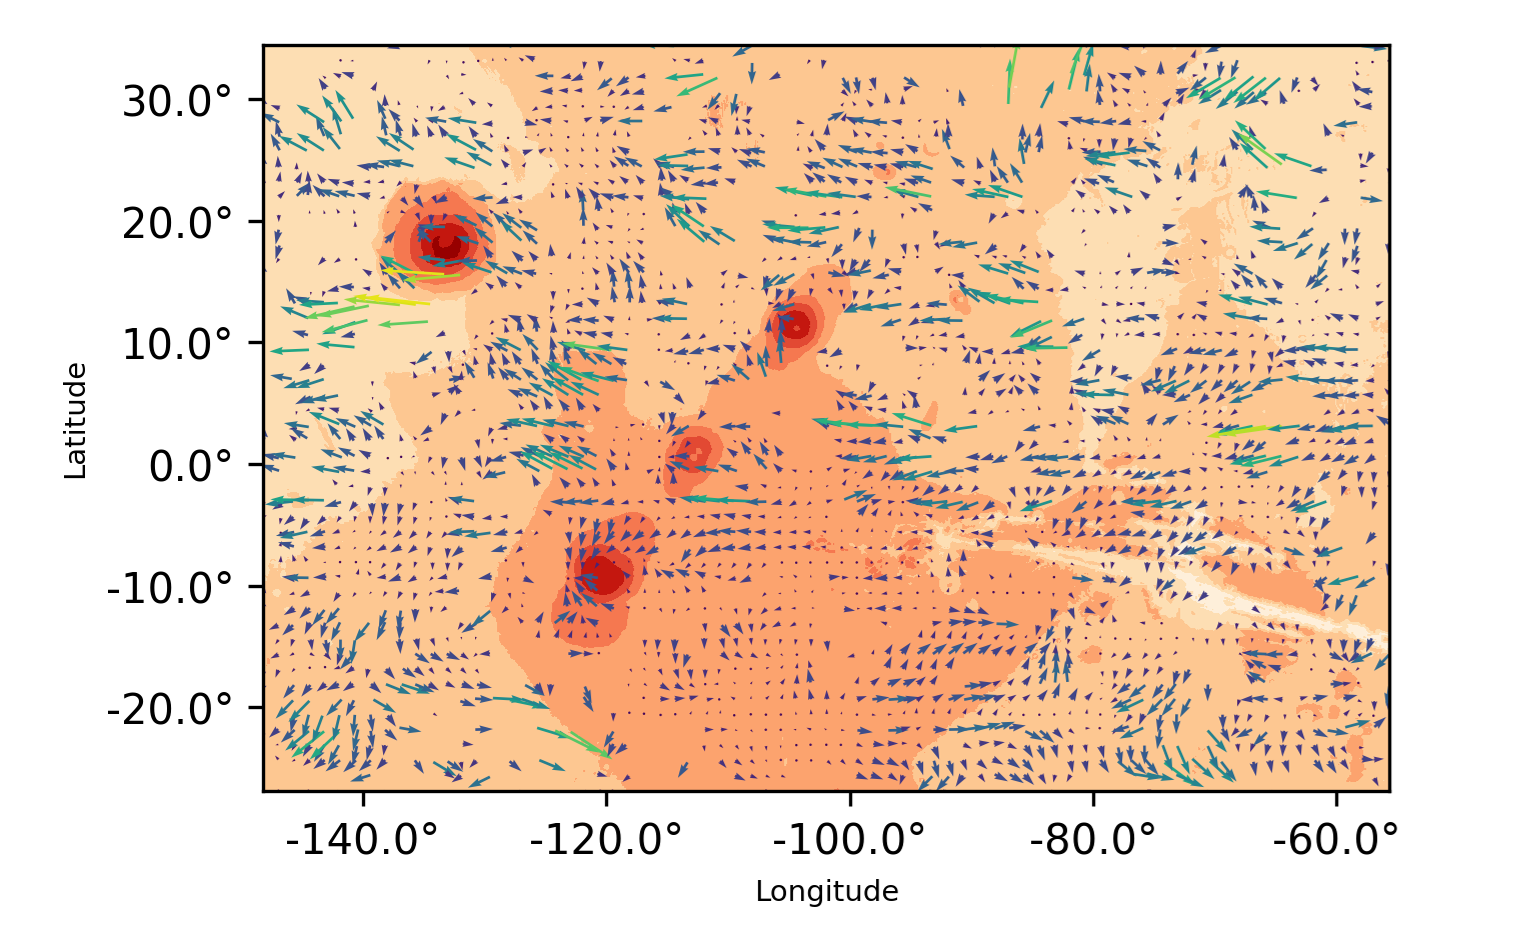
\includegraphics[width=1\textwidth]{fig_35.png}
    \caption{Velocity fields - UTC: 22/11/2021 14:16:52 - 14:26:52}
\end{figure}
\FloatBarrier
\begin{figure}[h!] 
    \centering
    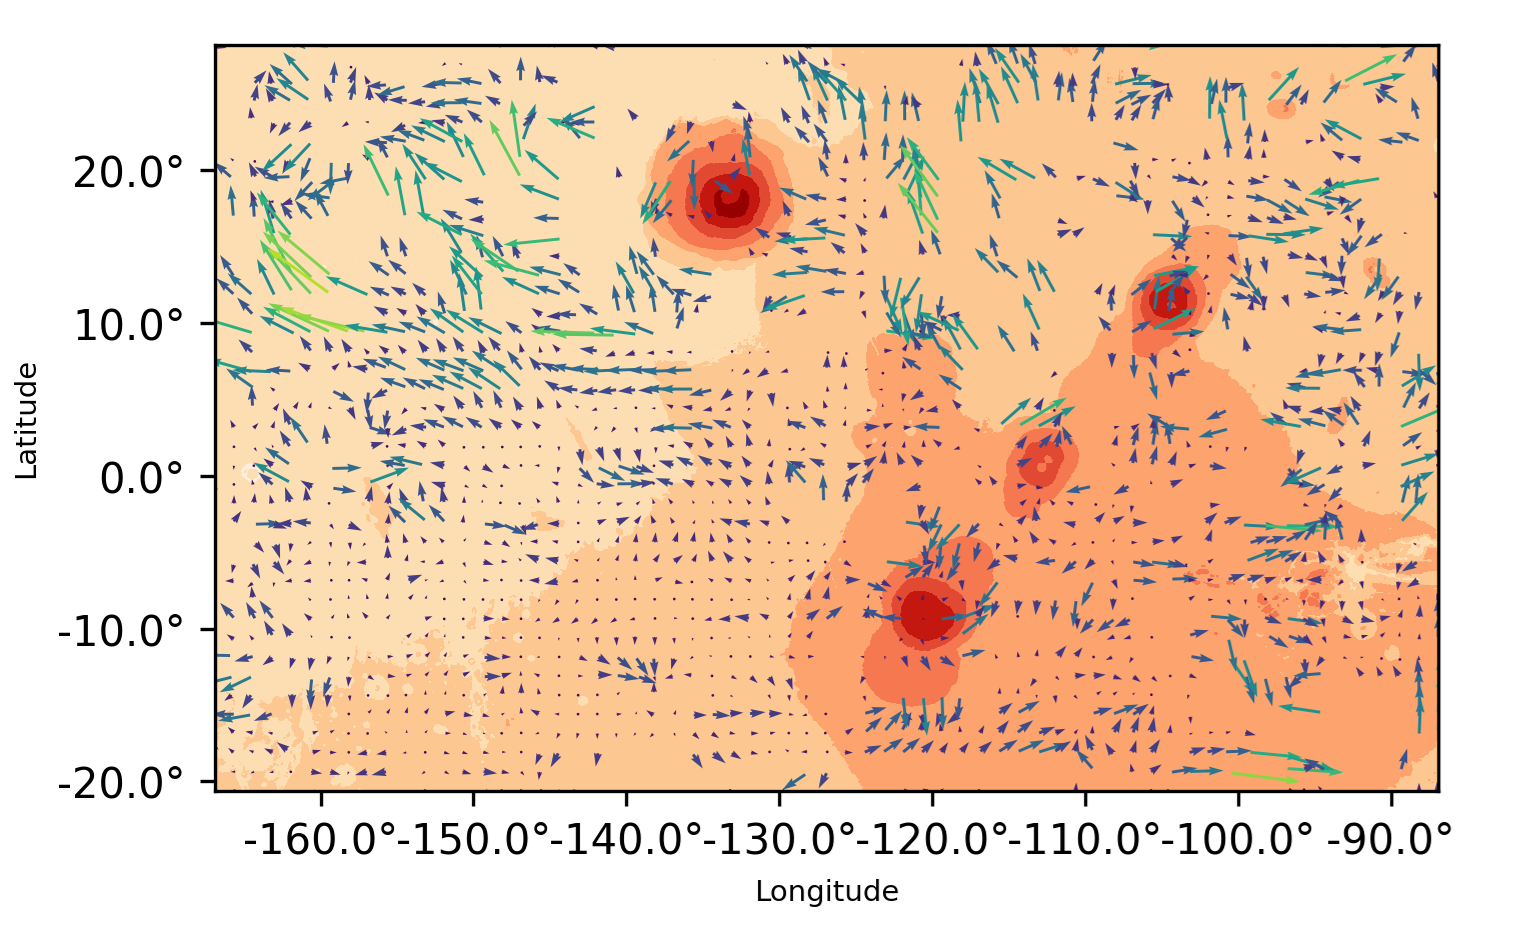
\includegraphics[width=1\textwidth]{fig_36.png}
    \caption{Velocity fields - UTC: 04/12/2021 00:31:53 - 00:41:53}
\end{figure}
\FloatBarrier
\begin{figure}[h!] 
    \centering
    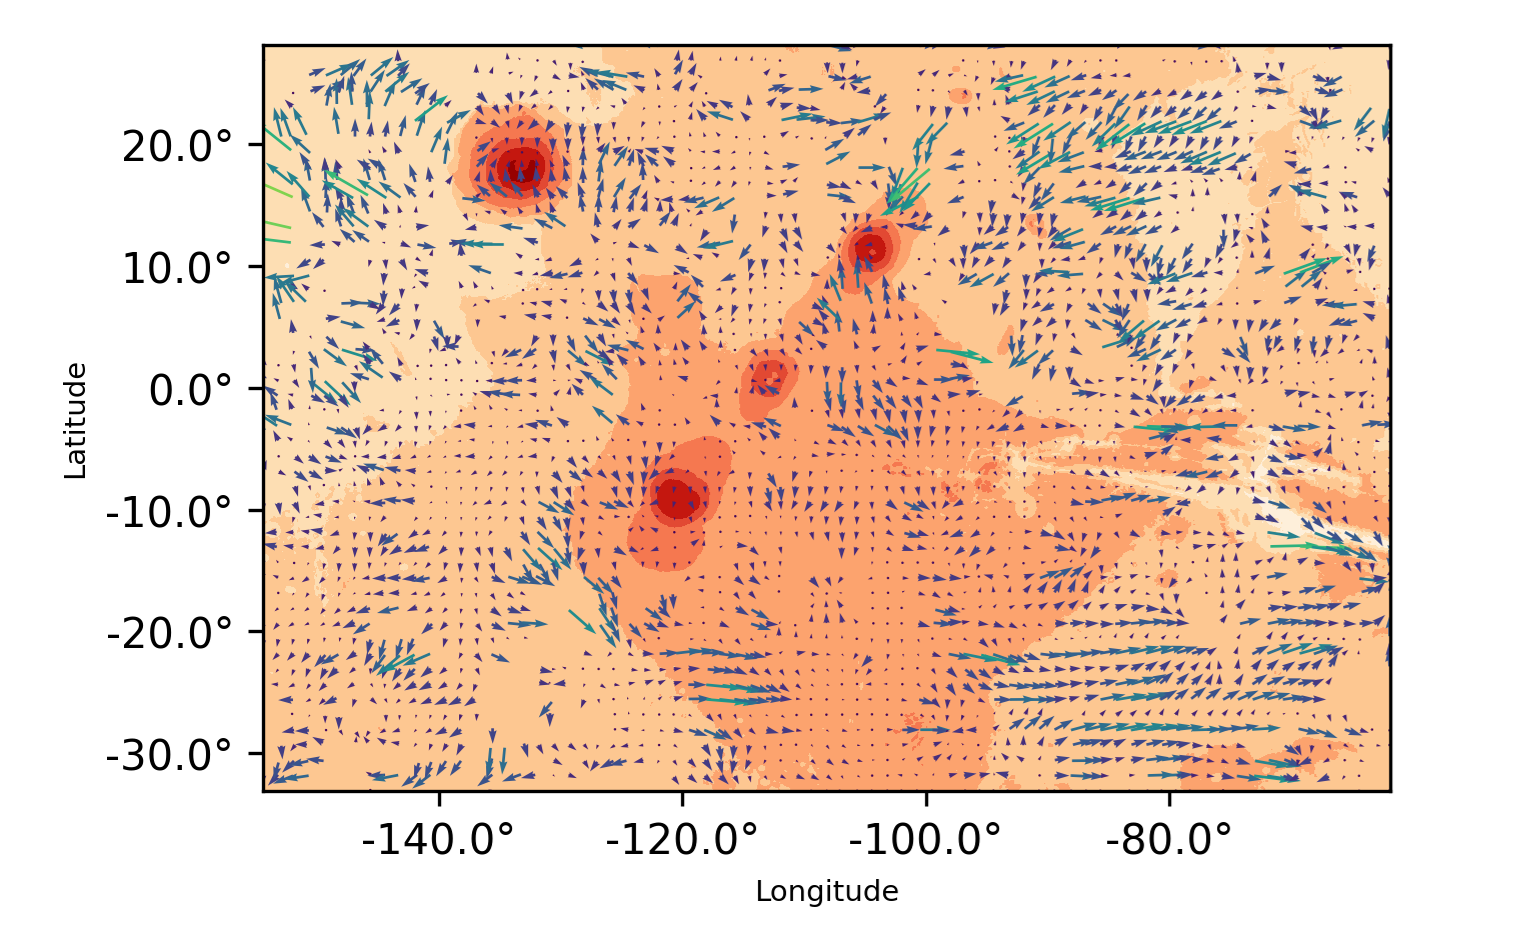
\includegraphics[width=1\textwidth]{fig_37.png}
    \caption{Velocity fields - UTC: 24/12/2021 10:30:07 - 10:40:06}
\end{figure}
\FloatBarrier
\begin{figure}[h!] 
    \centering
    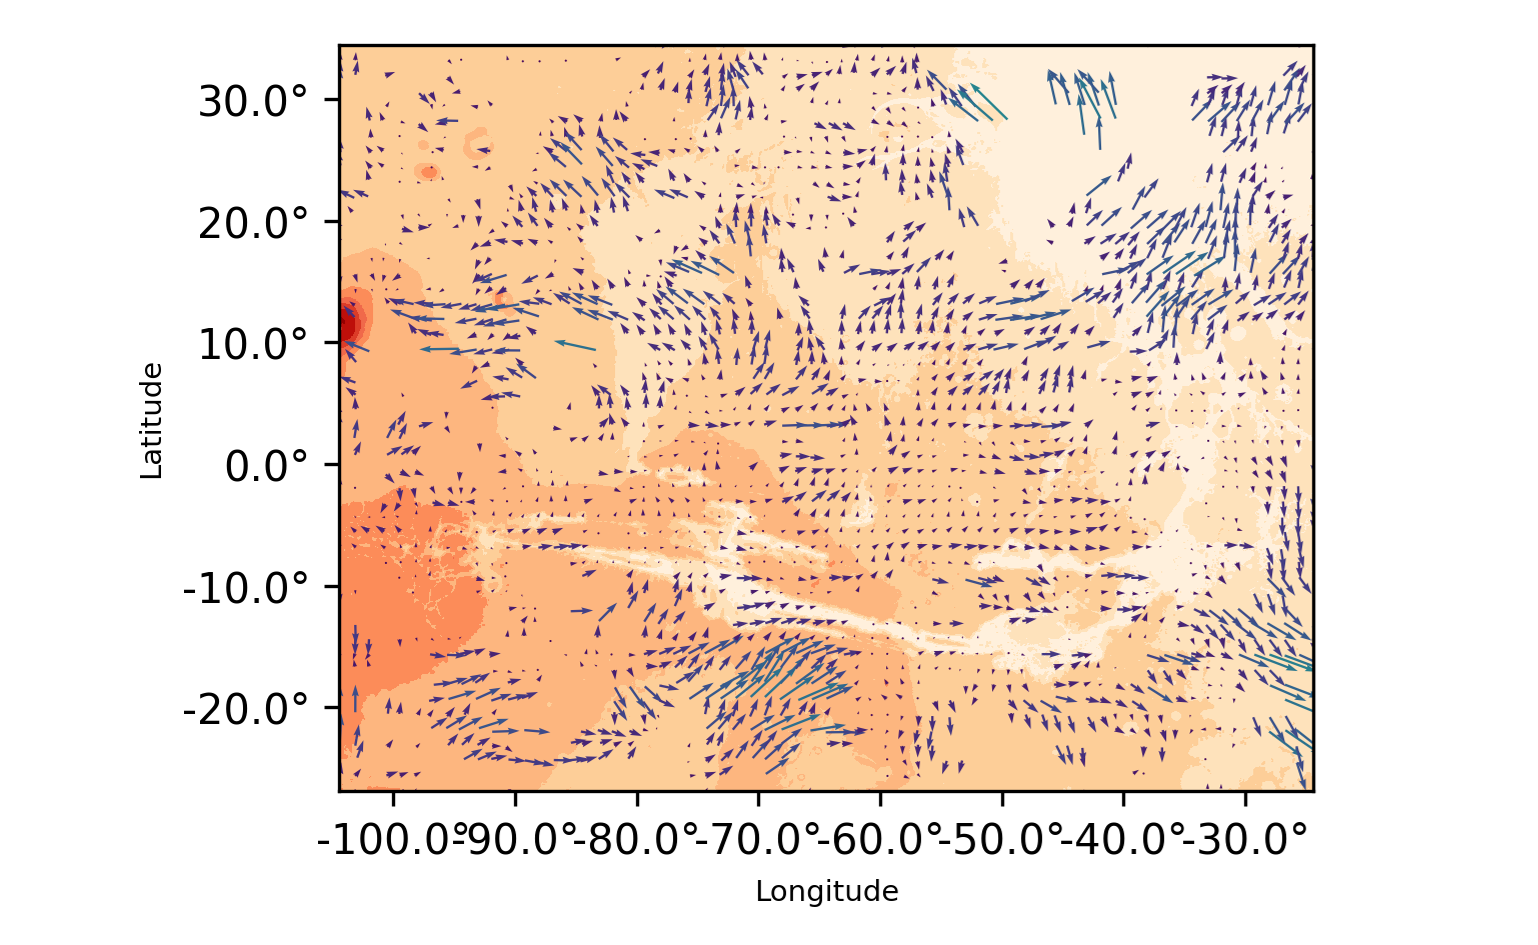
\includegraphics[width=1\textwidth]{fig_38.png}
    \caption{Velocity fields - UTC: 23/10/2023 05:40:13 - 06:10:16}
\end{figure}
\FloatBarrier
\begin{figure}[h!] 
    \centering
    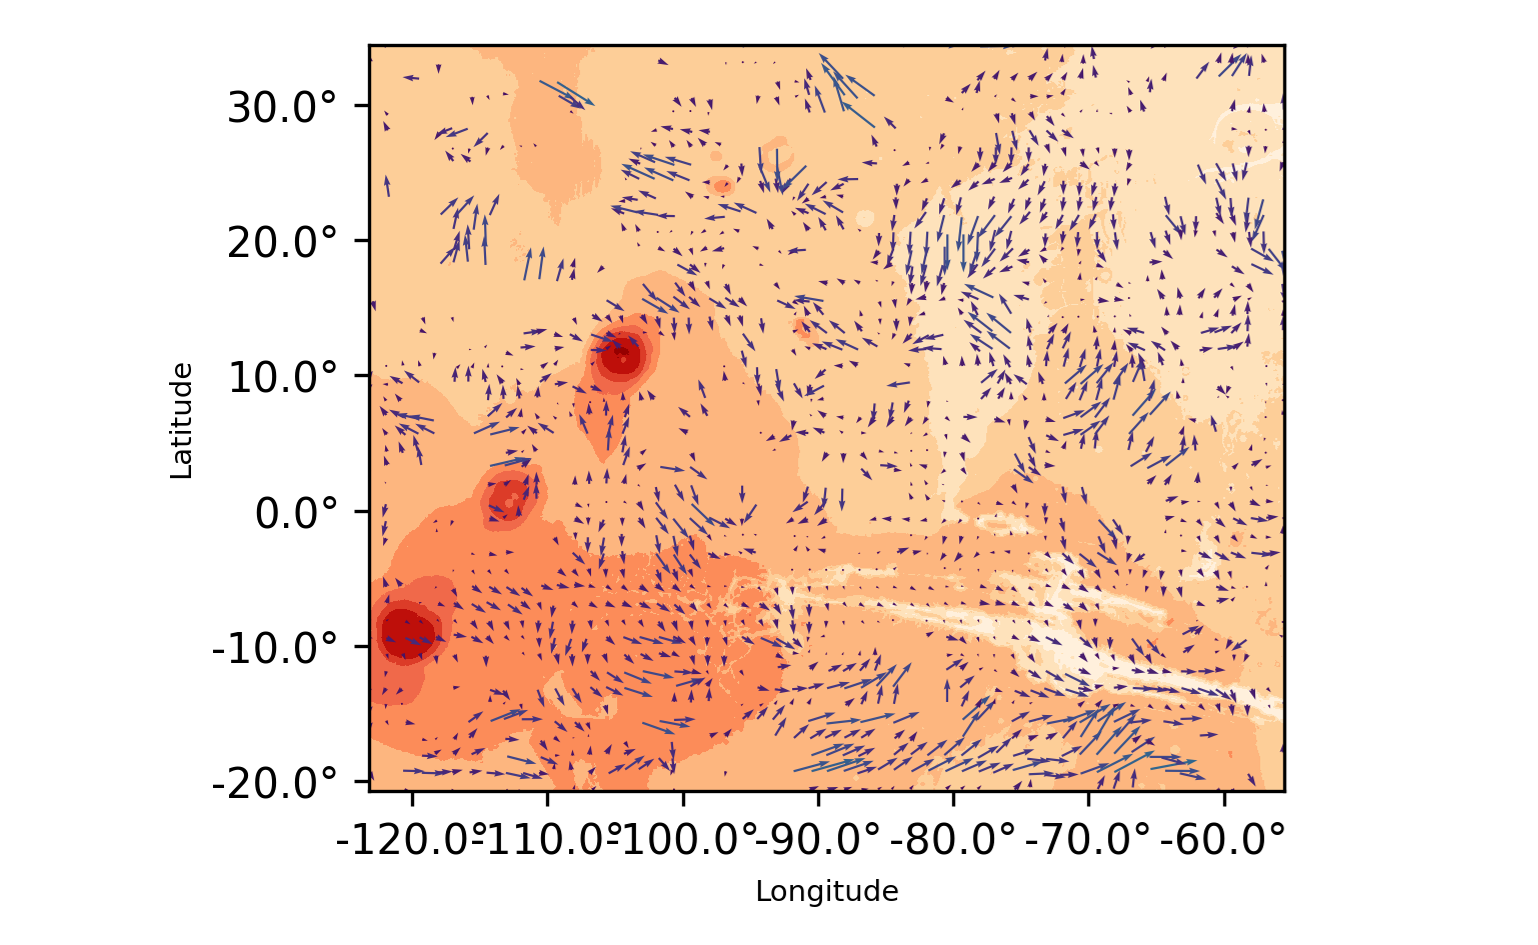
\includegraphics[width=1\textwidth]{fig_39.png}
    \caption{Velocity fields - UTC: 23/10/2023 08:18:33 - 08:48:36}
\end{figure}
\FloatBarrier
\begin{figure}[h!] 
    \centering
    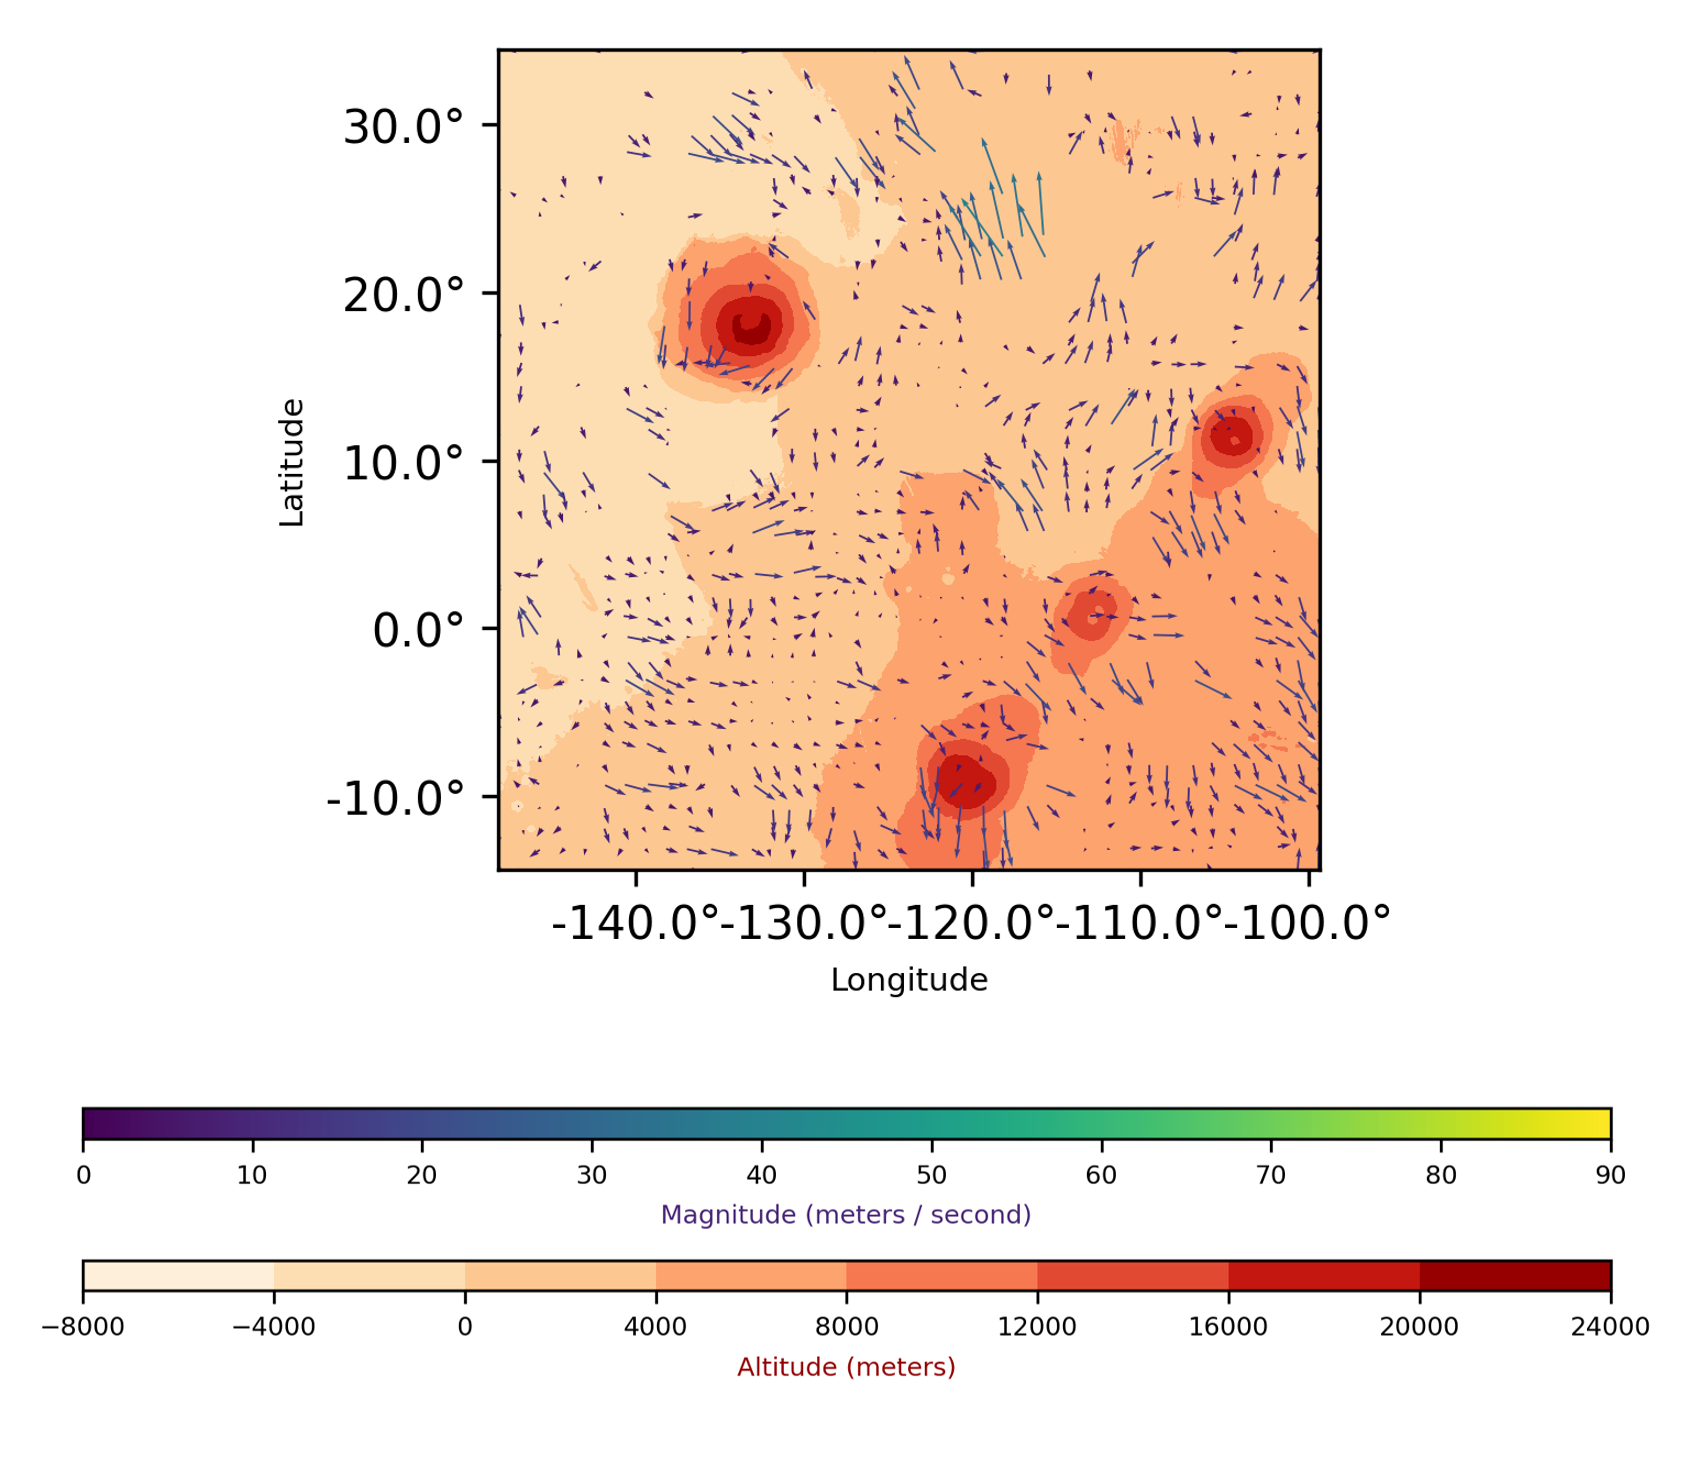
\includegraphics[width=1\textwidth]{fig_40.png}
    \caption{Velocity fields - UTC: 23/10/2023 10:56:50 - 11:26:53}
\end{figure}
\FloatBarrier
When comparing the wind fields in this thesis to those obtained by Shaimaa Ahmed AlBlooki in 2023 \cite{AlBlooki2023}, using a version of the data without pointing correction, some differences are noticeable. The wind field visualisations in this thesis display fewer vectors, potentially due to a higher correlation cut-off of 0.4 and different CIV parameters. Additionally, there are minor variations in vector locations, with some vectors present in Shaimaa Ahmed AlBlooki's results not appearing in this thesis’s wind fields, and the wind speeds in the 2023 thesis seem higher. Nevertheless, the overall wind directions remain consistent across both sets of wind field maps(see Figure 4.11).
\FloatBarrier
\begin{figure}[h!] 
    \centering
    \includegraphics[width=1\textwidth]{fig_41.png}
    \caption{Comparison of a wind field obtained in Shaimaa Ahmed AlBlooki 2023 thesis and this thesis - UTC: 22/11/2021 14:26:52 - 14:36:52}
\end{figure}
\FloatBarrier
Several trends are evident in the wind field visualizations (refer to Figure A.3 to A.8 for the complete sequences). In the northern hemisphere, winds tend to shift towards the northwest, particularly in the area left to approximately -140° longitude, near Olympus Mons. In contrast, winds in the southern hemisphere predominantly move southward. Additionally, in the southern hemisphere between longitudes of about -125° and -100°, there is a tendency for winds to shift towards the east.
Although wind speeds are generally higher in the Northern Hemisphere, there appears to be a pattern of symmetry in the wind field directions. This pattern suggests a possible mirrored symmetry relative to the equator, with a reversed orientation. The tendency for winds to shift northwards in the northern hemisphere and southwards in the southern hemisphere is also evident in the meridional plots shown in Figure A.2.